% ICASSP 2027 submission. Built with spconf.sty and IEEEbib.bst from this folder.
% Figures live in images/ and are regenerated by make_figures.py from the experiment results.
% --------------------------------------------------------------------------------------------
\documentclass{article}
\usepackage{spconf,amsmath,amssymb,graphicx,booktabs,cite}
% spconf loads Times via the "times" package, which only works under pdfLaTeX.
% Under XeLaTeX/LuaLaTeX use the Times clone TeX Gyre Termes instead.
\usepackage{iftex}
\ifPDFTeX\else
  \usepackage{fontspec}
  \setmainfont{texgyretermes}[Extension=.otf, UprightFont=*-regular, BoldFont=*-bold,
    ItalicFont=*-italic, BoldItalicFont=*-bolditalic]
\fi
\usepackage[hidelinks]{hyperref}
\usepackage{xurl}

\title{Is the acoustic codebook the bottleneck? Equivalence-bounded evidence from XLS-R on Sinhala and Tamil}

\name{Anas Hussaindeen, Ifadha Imthiyas, Vihanga Muthumala, Samadhi Talagala, Uthayasanker Thayasivam}
\address{Department of Computer Science and Engineering, University of Moratuwa, Sri Lanka \\
\texttt{\{anas.22, ifadha.22, vihangamuthumala.22,} \\
\texttt{samadhi.22, rtuthaya\}@cse.mrt.ac.lk}}

\begin{document}
\maketitle

\begin{abstract}
A common explanation for the weakness of self-supervised speech models on low-resource languages is that the frozen discrete codebook, learned mostly from high-resource speech, lacks units for their sounds. We test this for Sinhala and Tamil with XLS-R in three pre-registered studies. First, we show that the usual quantization residual is undefined for wav2vec~2.0-style quantizers and that its unmasked substitute is insensitive; measured at masked positions, both languages are fit at least as well as English. Second, across 18 FLEURS languages in nine family-matched pairs, the effect of pre-training membership is statistically equivalent to zero within a margin calibrated on perturbations known to degrade the codebook. Third, layer-wise linear probing at an exactly matched 3-hour budget shows the same depth profile for all three languages and no saturation. The one language-specific signal is higher probe instability at the best layers, which we cannot yet attribute to language rather than corpus.
\end{abstract}

\begin{keywords}
self-supervised speech representations, low-resource speech recognition, vector quantization, layer-wise probing, equivalence testing
\end{keywords}

\section{Introduction}
\label{sec:intro}

Self-supervised models such as wav2vec~2.0~\cite{baevski2020wav2vec} and HuBERT~\cite{hsu2021hubert} learn speech representations from untranscribed audio and are now a default starting point for low-resource automatic speech recognition (ASR)~\cite{mohamed2022review}. Their multilingual variants XLSR-53~\cite{conneau2021xlsr} and XLS-R~\cite{babu2022xlsr} nonetheless leave a wide gap between high- and low-resource languages, and fine-tuned XLS-R is known to lean on the languages that dominate its pre-training data~\cite{storey2024bias}. For wav2vec~2.0-style models an obvious suspect is the product quantizer: its codebook is learned jointly with the encoder on that skewed data, so a scarce or absent language might find no discrete units near its sounds. If so, extending or adapting the codebook would be a direct remedy. This paper is about that quantizer, so its claims are scoped to product-quantized models; HuBERT-family objectives have no comparable codebook and are not tested here.

We test that premise for Sinhala and Tamil before building on it. Our contributions are:
\begin{itemize}
\item We show that the quantization residual commonly assumed for this question is undefined for wav2vec~2.0, that its unmasked substitute barely responds even to white noise, and that masked-position contrastive metrics give a calibrated alternative (Sec.~\ref{sec:fit}).
\item On 4,999 clips with five positive controls, Sinhala and Tamil are fit at least as well as English (Sec.~\ref{sec:fit}).
\item Across 18 languages in nine family-matched pairs, the effect of pre-training membership is statistically equivalent to zero within a margin calibrated on codebook-degrading perturbations (Sec.~\ref{sec:membership}).
\item Layer-wise probing at an exactly matched budget finds a shared depth profile and no saturation; the only language-specific effect is probe instability at the best layers (Sec.~\ref{sec:layers}).
\item Fine-tuning the same model on the same matched budget halves or better the frozen-probe error in every language, placing the limit on adaptation and labelled data rather than on the representation (Sec.~\ref{sec:finetune}).
\end{itemize}
Decision criteria for every study were fixed in configuration files before results were computed.

\section{Relation to prior work}
\label{sec:prior}

Analyses of wav2vec~2.0 show that its discrete latents specialise to phonetic categories on English~\cite{baevski2020wav2vec}, and that intermediate transformer layers carry most phonetic and word information while early layers retain speaker and acoustic detail~\cite{pasad2021layerwise,pasad2023comparative}. SUPERB~\cite{yang2021superb} evaluates frozen representations with lightweight heads, including the learnable weighted sum over layers that we adopt. Probing studies caution that probe accuracy conflates representation and probe capacity and must be read against controls~\cite{hewitt2019control,belinkov2022probing}; this motivates our linear probes, random-initialisation floors and positive controls. Closer to our question, analyses of the discrete units ask whether they are language-specific or language-universal~\cite{abdullah2023discrete} and how codebook entries separate languages, varieties and speaking styles~\cite{linke2023encode}. The remedies that follow from a codebook deficit have also been explored: continued pre-training is reported to reshape the learned codeword groups for a target language~\cite{getman2024cpt}, and adapters add languages without retraining the quantizer~\cite{kessler2022adapter}. Our contribution is to test the premise those remedies assume rather than to propose another. Work on Sinhala and Tamil ASR~\cite{akhilesh2022tamil,icon2021sinhala,ilyas2026sinhala}, and on XLS-R for other under-resourced languages~\cite{nandi2021large}, reports downstream accuracy: \emph{whether} performance lags, not \emph{where} a deficit arises. We instead test the codebook hypothesis directly, and we support absence claims with equivalence tests~\cite{schuirmann1987tost,lakens2017equivalence}, which are rare in speech research but required before a non-significant result can be read as evidence of no effect.

\section{Codebook fit}
\label{sec:fit}

\subsection{Measurement}

In XLS-R~0.3B the convolutional encoder emits $\mathbf{z}_t\in\mathbb{R}^{512}$, and a Gumbel-softmax~\cite{jang2017gumbel} product quantizer selects one of $V{=}320$ codevectors in each of $G{=}2$ groups, concatenated into $\mathbf{q}_t\in\mathbb{R}^{768}$. The codevectors are free parameters that are never trained to reconstruct $\mathbf{z}_t$, so the vector-quantization residual $\|\mathbf{z}_t-\mathbf{q}_t\|^2$ is undefined. The natural substitute, the cosine distance between the projected context and the projected target at \emph{unmasked} frames, is nearly insensitive: it differs by only $1.11\times$ between clean English and white noise, because pre-training aligns the two only where the input is masked.

We therefore evaluate the pre-training objective itself. Under pre-training conditions (mask probability 0.065, span 10, $K{=}100$ distractors, temperature 0.1) we compute, at masked frames, the InfoNCE loss and the gap between the cosine similarity to the true target and the mean similarity to distractors, over three mask draws per file. Statistics are aggregated per file, and codebook-usage statistics exclude frames below 10\% of each file's 90th-percentile RMS.

\subsection{Data and controls}

We use 1,000 clips each of in-the-wild Sinhala and Tamil (YouTube), read Sinhala (OpenSLR-52~\cite{kjartansson2018crowd}), read Tamil (OpenSLR-65~\cite{he2020open}) and read English (Common Voice~\cite{ardila2020commonvoice}), truncated to 30\,s; the read arms hold speaking style roughly constant. Five positive controls of 300 clips each are derived from the English clips: 1.45$\times$ speed/pitch shift, six-way babble, time reversal, sine chirps and level-matched white noise.

\begin{table}[t]
\caption{Masked-position codebook fit on XLS-R 0.3B. Lower InfoNCE and a larger positive--negative gap indicate better fit; ratios are relative to English. Italic rows are positive controls built from the English clips. Chance InfoNCE is $\ln 101 = 4.62$.}
\label{tab:fit}
\vspace{3pt}
\centering\small
\setlength{\tabcolsep}{5pt}
\begin{tabular}{lrrrr}
\toprule
Condition & InfoNCE & $\times$EN & Gap & $\times$EN \\
\midrule
English, Common Voice & 2.829 & 1.00 & 0.453 & 1.00 \\
Sinhala, YouTube      & 2.085 & 0.74 & 0.540 & 1.19 \\
Tamil, YouTube        & 1.955 & 0.69 & 0.559 & 1.24 \\
Sinhala, read         & 2.632 & 0.93 & 0.489 & 1.08 \\
Tamil, read           & 2.678 & 0.95 & 0.484 & 1.07 \\
\midrule
\emph{Speed/pitch 1.45$\times$} & 3.118 & 1.10 & 0.419 & 0.93 \\
\emph{Six-way babble}           & 3.135 & 1.11 & 0.334 & 0.74 \\
\emph{Time reversal}            & 3.419 & 1.21 & 0.328 & 0.72 \\
\emph{Sine chirps}              & 3.816 & 1.35 & 0.351 & 0.77 \\
\emph{White noise}              & 4.852 & 1.71 & 0.010 & 0.02 \\
\bottomrule
\end{tabular}
\end{table}

\subsection{Results}

Table~\ref{tab:fit} shows that the masked metrics respond strongly to corruption---white noise drives InfoNCE to chance and collapses the gap---while Sinhala and Tamil sit on the favourable side of English in both recording conditions. Codebook usage is less diverse for Sinhala and Tamil (perplexity 0.73--0.95$\times$ English at matched frame budgets), but combined with an equal or better contrastive fit this indicates concentrated rather than failed coding; every language, English included, uses about 30\% of the entries in each group.

Repeating the analysis on XLSR-53 yields a natural experiment: its pre-training included Tamil but not Sinhala~\cite{conneau2021xlsr}, yet the two behave alike (InfoNCE $0.88\times$ and $0.82\times$ English on YouTube audio, $1.01\times$ and $1.03\times$ on read speech).

\section{Pre-training membership}
\label{sec:membership}

\subsection{Design}

To test whether this generalises, we paired 18 FLEURS~\cite{conneau2023fleurs} languages by family, one seen and one unseen by XLSR-53 per pair, with membership taken from the constituent corpus lists of MLS~\cite{pratap2020mls}, Common Voice and BABEL~\cite{conneau2021xlsr}: Bengali/Marathi, Polish/Czech, Persian/Greek, Estonian/Finnish, Kazakh/Uzbek, Tamil/Malayalam, Indonesian/Javanese, Mandarin/Burmese and Zulu/Xhosa. FLEURS reads the same FLoRes-101~\cite{goyal2022flores} sentences in every language, removing the domain confound of Sec.~\ref{sec:fit}. We scored 500 test clips per language on XLSR-53 and tested the nine within-pair differences in language-mean InfoNCE (unseen $-$ seen) with a Wilcoxon signed-rank test and with two one-sided tests (TOST)~\cite{schuirmann1987tost,lakens2017equivalence}. With nine pairs the minimum detectable effect at 80\% power is $d_z{=}1.07$.

The equivalence margin $\pm0.289$ is the InfoNCE increase caused by the mildest positive control in Table~\ref{tab:fit}. Clip duration lowers InfoNCE (median per-language Spearman $\rho=-0.36$) and mean FLEURS clip length differs by up to 68\% across languages, so we pre-registered both a full-clip analysis and fixed-window crops. Two windows were run because the registered 9\,s window discarded short clips unevenly (4--48\% per language); a 6\,s window retains 90--100\%.

\begin{figure}[t]
  \centering
  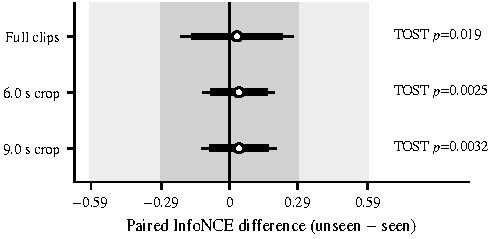
\includegraphics[width=\linewidth]{images/fig_equivalence}
  \caption{Paired InfoNCE difference (unseen $-$ seen) over nine family-matched pairs on XLSR-53. Thick bars: 90\% CI; thin bars: 95\% CI. Dark and light bands: equivalence margins from the speed/pitch ($\pm0.289$) and time-reversal ($\pm0.590$) controls.}
  \label{fig:equiv}
\end{figure}

\subsection{Results}

Figure~\ref{fig:equiv} shows paired differences of $+0.033$, $+0.040$ and $+0.041$ ($d_z=0.11$--$0.21$; Wilcoxon $p\geq0.57$) in the three regimes, with every 90\% confidence interval inside the margin (TOST $p=0.019$, $0.0025$ and $0.0032$). In every regime five pairs favour the seen language and four the unseen one. The same split applied to XLS-R~0.3B, which saw 18 of the 19 languages, gives $d_z=-0.01$ ($p=1.00$), as a negative control should. XLS-R pre-training hours show no association with fit among the twelve languages with 33--321\,h ($\rho=-0.01$, $p=0.97$); the weak association over the full range is carried by six languages above 5,000\,h, all European or English, and cannot be separated from region.

\section{Layer-wise probing}
\label{sec:layers}

\subsection{Setup}

We probe all 24 transformer layers of frozen XLS-R~0.3B for Sinhala (OpenSLR-52), Tamil (OpenSLR-65) and English (Common Voice), using exactly 3.00\,h of training and 0.50\,h of test audio per language from 40 speakers, with speaker-disjoint splits for the ASR probe. A linear layer trained with CTC~\cite{graves2006ctc} over characters (learning rate $10^{-2}$, batch 32, 25 epochs, AdamW) serves as the ASR probe; a linear classifier on mean-pooled features, trained on three utterances per speaker, identifies speakers. Each configuration uses three seeds. Because character error rate (CER) depends on the script, with inventories of 106, 49 and 34 characters, we compare only curve shape: each language's CER is normalised by its own best layer, and the pre-registered criterion for a depth-localised penalty was a shift, relative to English, of at least three layers in the best layer or two in the inverse-CER-weighted depth centroid. Transcripts were screened for implausible character rates (above 25 characters per second), a check that exposed and led us to fix a transcript-parsing error in an early Common Voice Tamil run.

A minority of CTC probe initialisations converge to degenerate solutions. We detect them from training loss alone, as runs whose final-to-initial loss ratio exceeds three times the best ratio in the same configuration, and replace them with fresh seeds.

\begin{figure}[t]
  \centering
  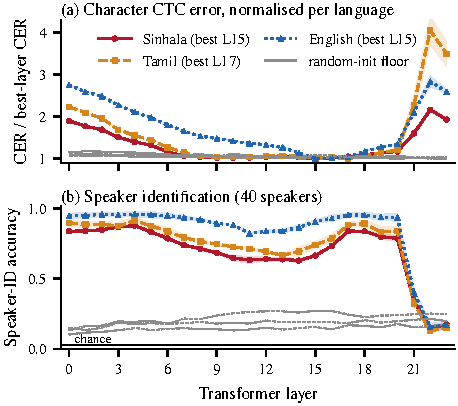
\includegraphics[width=\linewidth]{images/fig_layers}
  \caption{Layer profiles of frozen XLS-R 0.3B. (a) CTC character error rate normalised by each language's best layer. (b) Speaker-identification accuracy. Shaded bands: $\pm1$ SD over three seeds. Dotted grey: randomly initialised model of the same architecture.}
  \label{fig:layers}
\end{figure}

\begin{table}[t]
\caption{Layer probes and fine-tuning, all at the same 3\,h budget. $L^{*}$: best layer. Absolute CER is script-dependent and is compared only within a language. Fine-tuned: mean of three seeds. Collapse: degenerate linear-probe runs among nine seeds at eight layers.}
\label{tab:layers}
\vspace{3pt}
\centering\footnotesize
\setlength{\tabcolsep}{3.2pt}
\begin{tabular}{lrrrrrr}
\toprule
 & & CTC & Speaker ID & \multicolumn{2}{c}{Frozen CER at $L^{*}$} & \\
\cmidrule(lr){5-6}
Language & Chars & $L^{*}$ & $L^{*}$ (acc.) & 0.5\,h & 3\,h & Fine-tuned \\
\midrule
Sinhala & 106 & 15 & 4 (0.878) & 0.315 & 0.275 & 0.129 \\
Tamil   &  49 & 17 & 4 (0.914) & 0.215 & 0.170 & 0.062 \\
English &  34 & 15 & 4 (0.960) & 0.263 & 0.221 & 0.093 \\
\bottomrule
\end{tabular}
\end{table}

\subsection{Results}

Two validation checks pass (Fig.~\ref{fig:layers}). Probes on a randomly initialised copy of the model, trained on 1\,h, remain at CER 0.76--0.85 with no depth structure, and speaker identity peaks at layer 4 while character information peaks at layers 15--17 in every language, matching prior layer-wise analyses~\cite{pasad2021layerwise,pasad2023comparative}. The depth profiles agree (Table~\ref{tab:layers}): best layers differ from English by 0 and 2 layers and centroids by 0.7 and 0.8, so neither language meets the criterion. Tamil's curve is more sharply peaked, a descriptive statistic that was not pre-registered. A SUPERB-style weighted sum~\cite{yang2021superb} over all layers improves on the best single layer for every language (CER 0.260, 0.164 and 0.211 against 0.273, 0.170 and 0.219).

Speaker accuracy, the one metric comparable across languages, is lower for Tamil and Sinhala than for English. The gap is already present at layer 0 and does not grow with depth ($\rho\approx0$), which points to differences between the corpora rather than the representation: Common Voice contributors record on their own devices, which can make speakers separable by channel, and Sinhala clips are the shortest. Retraining the best-layer CTC probe on 0.5, 1, 2 and 3\,h lowers CER monotonically in all three languages, with no plateau at 3\,h.

Probe \emph{stability}, however, does differ. Across nine independent initialisations at eight layers, CTC probes collapsed in 12 of 144 runs for Sinhala and Tamil and in none of 72 for English (Fisher $p=0.010$). Collapses concentrated at layers 15 and 17 (22\% against 4\% elsewhere, $p=0.002$), but that comparison was chosen after the best layers were known and is uncorrected. Discarding collapsed runs changed CER at those layers by at most 0.003, so the shape comparison is unaffected. A Common Voice Tamil arm (22 speakers, best CER 0.251) collapsed in 4 of 72 runs, statistically indistinguishable from both OpenSLR Tamil ($p=0.53$) and Common Voice English ($p=0.12$); pooled comparisons lean toward language, but we cannot yet attribute the instability to language rather than corpus.

\subsection{Fine-tuning}
\label{sec:finetune}

Frozen probes bound what a linear head can read off a representation, not what the model achieves once adapted. We therefore fine-tuned the same checkpoint with a CTC head on exactly the same splits, budget, vocabularies and seeds, freezing only the CNN feature encoder (lr $10^{-4}$, batch 8, 30 epochs); the sole change is that the encoder trains. This arm was added after review and is not part of the pre-registered protocol.

Fine-tuning lowers CER against the 3\,h frozen column of Table~\ref{tab:layers} by 53\%, 64\% and 58\% relative for Sinhala, Tamil and English, reaching $0.129\pm0.006$, $0.062\pm0.003$ and $0.093\pm0.003$ over three seeds. Two things follow. At this budget the frozen representation is not what limits any of the three languages, which supports reading the probe results as data- and adaptation-limited. And the ordering is unchanged---Tamil, then English, then Sinhala, both frozen and fine-tuned---so adaptation neither creates nor removes a low-resource penalty; the residual spread tracks script and corpus, Sinhala carrying the largest character inventory and the shortest clips. None of the nine fine-tuning runs collapsed, in contrast to the linear probes.

\section{Discussion and limitations}
\label{sec:discussion}

Across three levels of analysis we find no evidence that XLS-R's codebook, its pre-training language coverage, or any particular depth disadvantages Sinhala or Tamil relative to English. At a 3\,h labelled budget none of the probes has saturated and fine-tuning more than halves their error, so the binding constraint here is labelled data and adaptation rather than the representation; whether the representation becomes limiting at larger budgets is untested. For the motivating application this argues against extending the acoustic codebook.

The evidence has clear limits. Apart from the YouTube arm of Sec.~\ref{sec:fit}, all audio is read speech, whereas practical systems face spontaneous recordings. Language and corpus are confounded throughout, and our one attempt to separate them was inconclusive. The equivalence margin is calibrated on unpaired, cross-corpus controls on XLS-R~0.3B and transferred to paired differences on XLSR-53, so it is an anchor rather than a formally matched margin; the XLSR-53 control would give a more lenient 0.327. Samples are small, with nine pairs and three probing languages, and CER cannot be compared across scripts. Probe collapse at the \emph{best} layers is unexplained: a sharper optimum in a more rugged loss surface, or trivial convergence at uninformative layers, would each produce it.

\section{Conclusion}
\label{sec:conclusion}

XLS-R's frozen acoustic codebook does not under-represent Sinhala or Tamil: both are fit at least as well as English, pre-training membership has an equivalence-bounded null effect across 18 languages, the layer-wise profile is shared with English, and fine-tuning at the same budget more than halves the frozen-probe error in every language. Efforts to improve these languages should look beyond codebook extension, and claims of representational deficits should be tested against positive controls and equivalence bounds. Code, pre-registered configurations and per-file results are available at \url{https://github.com/EchoVerge-Labs/XLR-S-codebook-experiment}.

{\ninept
\bibliographystyle{IEEEbib}
\bibliography{references}}

\end{document}
